%---------------
%╔═╗╔═╗╔╦╗╦ ╦╔═╗
%╚═╗║╣  ║ ║ ║╠═╝
%╚═╝╚═╝ ╩ ╚═╝╩
%---------------

% language setup
\newcommand{\docLanguage}{ngerman}
%\newcommand{\docLanguage}{english}

% DOCUMENT SETUP
\documentclass[12pt, oneside, a4paper, \docLanguage]{report}
\usepackage[left=3cm,
			right=2.5cm,
			top=2.5cm,
			bottom=2.5cm,
			includehead,
			includefoot]{geometry}

% line spacing
\usepackage{setspace}
\setstretch{1,25} % 15/12 --> 1.25

% encoding setup
% T1 font encoding for languages that use a latin alphabet
\usepackage[T1]{fontenc}

% enhanced input encoding handling - utf8 for äÄüÜöÖß...
\usepackage[utf8]{inputenc}

%de­fines Adobe Times Ro­man as de­fault text font
\usepackage{mathptmx}
\usepackage{times} % needed for acronym package

%PDF linking package
\usepackage[hidelinks]{hyperref}


% Language Setup
\usepackage[\docLanguage]{babel}
% after babel - set chapter string
\AtBeginDocument{\renewcommand{\chaptername}{}}

% language specific bibliography style
\usepackage[numbers, square]{natbib}
%\setcitestyle{square,aysep={},yysep={;}}
\usepackage{babelbib}
% bliographystyle setup
% babel specific: babplain, babplai3, babalpha, babunsrt, bababbrv, bababbr3
\bibliographystyle{babunsrt}


% enumeration
\usepackage{enumitem}
% tabular extension tabularx
\usepackage{tabularx}

% math packages
\usepackage{amsmath}
\usepackage{nicefrac}
\usepackage{amsthm}
\usepackage{amsbsy}
\usepackage{amssymb}
\usepackage{amsfonts}
%\usepackage{MnSymbol}


%special characters
\usepackage{amssymb}
\usepackage{upgreek,textgreek}

% acronym package
\usepackage[printonlyused, footnote]{acronym}

% breakable text in \seqsplit{}
\usepackage{seqsplit}

% \textmu
\usepackage{textcomp}

% package provides a way to compile sections of a document using the same preamble as the main document
\usepackage{subfiles}

% driver-independent color extension - used by listings,tabularx
\usepackage[usenames,dvipsnames,table,xcdraw]{xcolor}

% -- SYNTAX HIGHLIGHTING --
\usepackage{listings}
%% bash command line Syntax Highlighting
\lstdefinestyle{BASH_CMD}{ 
  columns=fullflexible,            % copy pasteable listings
  language=bash,
  basicstyle=\small\sffamily,
  basicstyle   = \small \ttfamily,
  keywordstyle = [1]\small \ttfamily,
  keywordstyle = [2]\small \ttfamily,
  commentstyle = \small \ttfamily,
  numbers=none,
  captionpos=b, 
  breaklines=true,
  numberstyle=\tiny,
  numbersep=3pt,
  frame=tlrb,
  columns=fullflexible,
  backgroundcolor=\color{white!20},
  linewidth=\linewidth,
  literate=                        % replace in code
     {Ö}{{\"O}}1
     {Ä}{{\"A}}1
     {Ü}{{\"U}}1
     {ß}{{\ss}}2
     {ü}{{\"u}}1
     {ä}{{\"a}}1
     {ö}{{\"o}}1
}
 % adds style BASH_CMD
%% Matlab Syntax Highlighting
\colorlet{keyword}{blue!100!black!80}
\colorlet{STD}{Lavender}
\colorlet{comment}{green!90!black!90}
\definecolor{mygreen}{rgb}{0,0.6,0}
\definecolor{mygray}{rgb}{0.5,0.5,0.5}
\definecolor{mymauve}{rgb}{0.58,0,0.82}


\lstdefinestyle{BASH_SCRIPT}{ 
  language     = bash,
  basicstyle   = \footnotesize \ttfamily,
  keywordstyle = [1]\color{keyword}\bfseries,
  keywordstyle = [2]\color{STD}\bfseries,
  commentstyle = \color{mygreen}\itshape,
  backgroundcolor=\color{white},   % choose the background color; you must add \usepackage{color} 
  columns=fullflexible,            % copy pasteable listings
                                   % or \usepackage{xcolor}
  basicstyle=\footnotesize,        % the size of the fonts that are used for the code
  breakatwhitespace=false,         % sets if automatic breaks should only happen at whitespace
  breaklines=true,                 % sets automatic line breaking
  captionpos=b,                    % sets the caption-position to bottom
  extendedchars=true,              % lets you use non-ASCII characters; for 8-bits encodings only,
                                   % does not work with UTF-8
  frame=single,                    % adds a frame around the code
  keepspaces=true,                 % keeps spaces in text, useful for keeping indentation of code
                                   % (possibly needs columns=flexible)
  numbers=left,                    % where to put the line-numbers; possible values are 
                                   % (none, left, right)
  numbersep=5pt,                   % how far the line-numbers are from the code
  numberstyle=\tiny\color{mygray}, % the style that is used for the line-numbers
  rulecolor=\color{black},         % if not set, the frame-color may be changed on line-breaks
                                   % within not-black text (e.g. comments (green here))
  showspaces=false,                % show spaces everywhere adding particular underscores; it
  	                               % overrides 'showstringspaces'
  showstringspaces=false,          % underline spaces within strings only
  showtabs=false,                  % show tabs within strings adding particular underscores
  stepnumber=1,                    % the step between two line-numbers. If it's 1, each line 
                                   % will be numbered
  stringstyle=\color{mymauve},     % string literal style
  tabsize=2,                       % sets default tabsize to 2 spaces
  title=\lstname,                  % set title name
  literate=                        % replace in code
     {Ö}{{\"O}}1 
     {Ä}{{\"A}}1 
     {Ü}{{\"U}}1 
     {ß}{{\ss}}2 
     {ü}{{\"u}}1 
     {ä}{{\"a}}1 
     {ö}{{\"o}}1 
     {â}{{\^{a}}}1 
     {Â}{{\^{A}}}1 
     {ç}{{\c{c}}}1 
     {Ç}{{\c{C}}}1 
     {ğ}{{\u{g}}}1 
     {Ğ}{{\u{G}}}1 
     {ı}{{\i}}1 
     {İ}{{\.{I}}}1 
     {ş}{{\c{s}}}1 
     {Ş}{{\c{S}}}1 
} % adds style BASH_SCRIPT
% Matlab Syntax Highlighting
\colorlet{keyword}{blue!100!black!80}
\colorlet{STD}{red}
\colorlet{comment}{green!90!black!90}
\definecolor{mygreen}{rgb}{0,0.6,0}
\definecolor{mygray}{rgb}{0.5,0.5,0.5}
\definecolor{mymauve}{rgb}{0.58,0,0.82}


\lstdefinestyle{LATEX}{ 
  language     = [LaTeX]{TeX},
  basicstyle   = \footnotesize \ttfamily,
  keywordstyle = [1]\color{keyword}\bfseries,
  keywordstyle = [2]\color{comment}\bfseries,
  commentstyle = \color{mygray}\itshape,
  %backgroundcolor=\color{white},   % choose the background color; you must add \usepackage{color} 
                                   % or \usepackage{xcolor}
  basicstyle=\footnotesize,        		   % the size of the fonts that are used for the code
  breakatwhitespace=false,         % sets if automatic breaks should only happen at whitespace
  columns=fullflexible,            % copy pasteable listings
  breaklines=true,                 % sets automatic line breaking
  captionpos=c,                    % sets the caption-position to bottom
  extendedchars=true,              % lets you use non-ASCII characters; for 8-bits encodings only,
                                   % does not work with UTF-8
  frame=single,                    % adds a frame around the code
  keepspaces=true,                 % keeps spaces in text, useful for keeping indentation of code
                                   % (possibly needs columns=flexible)
  numbers=left,                    % where to put the line-numbers; possible values are 
                                   % (none, left, right)
  numbersep=4pt,                   % how far the line-numbers are from the code
  numberstyle=\tiny\color{mygray}, % the style that is used for the line-numbers
  rulecolor=\color{black},         % if not set, the frame-color may be changed on line-breaks
                                   % within not-black text (e.g. comments (green here))
  showspaces=false,                % show spaces everywhere adding particular underscores; it
  	                               % overrides 'showstringspaces'
  showstringspaces=false,          % underline spaces within strings only
  showtabs=false,                  % show tabs within strings adding particular underscores
  stepnumber=1,                    % the step between two line-numbers. If it's 1, each line 
                                   % will be numbered
  stringstyle=\color{mymauve},     % string literal style
  tabsize=2,                       % sets default tabsize to 2 spaces
  title=\lstname,                  % set title name
  literate=                        % replace in code
     {Ö}{{\"O}}1 
     {Ä}{{\"A}}1 
     {Ü}{{\"U}}1 
     {ß}{{\ss}}2 
     {ü}{{\"u}}1 
     {ä}{{\"a}}1 
     {ö}{{\"o}}1 
     {â}{{\^{a}}}1 
     {Â}{{\^{A}}}1 
     {ç}{{\c{c}}}1 
     {Ç}{{\c{C}}}1 
     {ğ}{{\u{g}}}1 
     {Ğ}{{\u{G}}}1 
     {ı}{{\i}}1 
     {İ}{{\.{I}}}1 
     {ş}{{\c{s}}}1 
     {Ş}{{\c{S}}}1 
} % adds style LATEX
%% Matlab Syntax Highlighting
\colorlet{keyword}{blue!100!black!80}
\colorlet{STD}{Lavender}
\colorlet{comment}{green!90!black!90}
\definecolor{mygreen}{rgb}{0,0.6,0}
\definecolor{mygray}{rgb}{0.5,0.5,0.5}
\definecolor{mymauve}{rgb}{0.58,0,0.82}


\lstdefinestyle{MATLAB}{ 
  language     = Matlab,
  basicstyle   = \footnotesize \ttfamily,
  keywordstyle = [1]\color{keyword}\bfseries,
  keywordstyle = [2]\color{STD}\bfseries,
  commentstyle = \color{mygreen}\itshape,
  backgroundcolor=\color{white},   % choose the background color; you must add \usepackage{color} 
                                   % or \usepackage{xcolor}
  basicstyle=\footnotesize,        % the size of the fonts that are used for the code
  breakatwhitespace=false,         % sets if automatic breaks should only happen at whitespace
  columns=fullflexible,            % copy pasteable listings
  breaklines=false,                % sets automatic line breaking
  captionpos=c,                    % sets the caption-position to bottom
  extendedchars=true,              % lets you use non-ASCII characters; for 8-bits encodings only,
                                   % does not work with UTF-8
  frame=single,                    % adds a frame around the code
  keepspaces=true,                 % keeps spaces in text, useful for keeping indentation of code
                                   % (possibly needs columns=flexible)
  numbers=left,                    % where to put the line-numbers; possible values are 
                                   % (none, left, right)
  numbersep=5pt,                   % how far the line-numbers are from the code
  numberstyle=\tiny\color{mygray}, % the style that is used for the line-numbers
  rulecolor=\color{black},         % if not set, the frame-color may be changed on line-breaks
                                   % within not-black text (e.g. comments (green here))
  showspaces=false,                % show spaces everywhere adding particular underscores; it
  	                               % overrides 'showstringspaces'
  showstringspaces=false,          % underline spaces within strings only
  showtabs=false,                  % show tabs within strings adding particular underscores
  stepnumber=1,                    % the step between two line-numbers. If it's 1, each line 
                                   % will be numbered
  stringstyle=\color{mymauve},     % string literal style
  tabsize=2,                       % sets default tabsize to 2 spaces
  title=\lstname,                  % set title name
  literate=                        % replace in code
     {Ö}{{\"O}}1 
     {Ä}{{\"A}}1 
     {Ü}{{\"U}}1 
     {ß}{{\ss}}2 
     {ü}{{\"u}}1 
     {ä}{{\"a}}1 
     {ö}{{\"o}}1 
     {â}{{\^{a}}}1 
     {Â}{{\^{A}}}1 
     {ç}{{\c{c}}}1 
     {Ç}{{\c{C}}}1 
     {ğ}{{\u{g}}}1 
     {Ğ}{{\u{G}}}1 
     {ı}{{\i}}1 
     {İ}{{\.{I}}}1 
     {ş}{{\c{s}}}1 
     {Ş}{{\c{S}}}1 
} % adds style MATLAB
% Matlab Syntax Highlighting
\colorlet{keyword}{blue!100!black!80}
\colorlet{STD}{Lavender}
\colorlet{comment}{green!90!black!90}
\definecolor{mygreen}{rgb}{0,0.6,0}
\definecolor{mygray}{rgb}{0.5,0.5,0.5}
\definecolor{mymauve}{rgb}{0.58,0,0.82}


\lstdefinestyle{PYTHON}{ 
  language     = Python,
  basicstyle   = \footnotesize \ttfamily,
  keywordstyle = [1]\color{keyword}\bfseries,
  keywordstyle = [2]\color{STD}\bfseries,
  commentstyle = \color{mygreen}\itshape,
  backgroundcolor=\color{white},   % choose the background color; you must add \usepackage{color} 
                                   % or \usepackage{xcolor}
  basicstyle=\footnotesize,        % the size of the fonts that are used for the code
  columns=fullflexible,            % copy pasteable listings
  breakatwhitespace=false,         % sets if automatic breaks should only happen at whitespace
  breaklines=false,                % sets automatic line breaking
  captionpos=c,                    % sets the caption-position to bottom
  extendedchars=true,              % lets you use non-ASCII characters; for 8-bits encodings only,
                                   % does not work with UTF-8
  frame=single,                    % adds a frame around the code
  keepspaces=true,                 % keeps spaces in text, useful for keeping indentation of code
                                   % (possibly needs columns=flexible)
  numbers=left,                    % where to put the line-numbers; possible values are 
                                   % (none, left, right)
  numbersep=5pt,                   % how far the line-numbers are from the code
  numberstyle=\tiny\color{mygray}, % the style that is used for the line-numbers
  rulecolor=\color{black},         % if not set, the frame-color may be changed on line-breaks
                                   % within not-black text (e.g. comments (green here))
  showspaces=false,                % show spaces everywhere adding particular underscores; it
  	                               % overrides 'showstringspaces'
  showstringspaces=false,          % underline spaces within strings only
  showtabs=false,                  % show tabs within strings adding particular underscores
  stepnumber=1,                    % the step between two line-numbers. If it's 1, each line 
                                   % will be numbered
  stringstyle=\color{mymauve},     % string literal style
  tabsize=2,                       % sets default tabsize to 2 spaces
  title=\lstname,                  % set title name
  literate=                        % replace in code
     {Ö}{{\"O}}1 
     {Ä}{{\"A}}1 
     {Ü}{{\"U}}1 
     {ß}{{\ss}}2 
     {ü}{{\"u}}1 
     {ä}{{\"a}}1 
     {ö}{{\"o}}1 
     {â}{{\^{a}}}1 
     {Â}{{\^{A}}}1 
     {ç}{{\c{c}}}1 
     {Ç}{{\c{C}}}1 
     {ğ}{{\u{g}}}1 
     {Ğ}{{\u{G}}}1 
     {ı}{{\i}}1 
     {İ}{{\.{I}}}1 
     {ş}{{\c{s}}}1 
     {Ş}{{\c{S}}}1 
} % adds style PYTHON
%% Matlab Syntax Highlighting
\colorlet{keyword}{blue!100!black!80}
\colorlet{STD}{Lavender}
\colorlet{comment}{green!90!black!90}
\definecolor{mygreen}{rgb}{0,0.6,0}
\definecolor{mygray}{rgb}{0.5,0.5,0.5}
\definecolor{mymauve}{rgb}{0.58,0,0.82}


\lstdefinestyle{CPP}{ 
  language     = C++,
  basicstyle   = \footnotesize \ttfamily,
  keywordstyle = [1]\color{keyword}\bfseries,
  keywordstyle = [2]\color{STD}\bfseries,
  commentstyle = \color{mygreen}\itshape,
  backgroundcolor=\color{white},   % choose the background color; you must add \usepackage{color} 
                                   % or \usepackage{xcolor}
  columns=fullflexible,            % copy pasteable listings
  basicstyle=\footnotesize,        % the size of the fonts that are used for the code
  breakatwhitespace=false,         % sets if automatic breaks should only happen at whitespace
  breaklines=false,                % sets automatic line breaking
  captionpos=c,                    % sets the caption-position to bottom
  extendedchars=true,              % lets you use non-ASCII characters; for 8-bits encodings only,
                                   % does not work with UTF-8
  frame=single,                    % adds a frame around the code
  keepspaces=true,                 % keeps spaces in text, useful for keeping indentation of code
                                   % (possibly needs columns=flexible)
  numbers=left,                    % where to put the line-numbers; possible values are 
                                   % (none, left, right)
  numbersep=5pt,                   % how far the line-numbers are from the code
  numberstyle=\tiny\color{mygray}, % the style that is used for the line-numbers
  rulecolor=\color{black},         % if not set, the frame-color may be changed on line-breaks
                                   % within not-black text (e.g. comments (green here))
  showspaces=false,                % show spaces everywhere adding particular underscores; it
  	                               % overrides 'showstringspaces'
  showstringspaces=false,          % underline spaces within strings only
  showtabs=false,                  % show tabs within strings adding particular underscores
  stepnumber=1,                    % the step between two line-numbers. If it's 1, each line 
                                   % will be numbered
  stringstyle=\color{mymauve},     % string literal style
  tabsize=2,                       % sets default tabsize to 2 spaces
  title=\lstname,                  % set title name
  literate=                        % replace in code
     {Ö}{{\"O}}1 
     {Ä}{{\"A}}1 
     {Ü}{{\"U}}1 
     {ß}{{\ss}}2 
     {ü}{{\"u}}1 
     {ä}{{\"a}}1 
     {ö}{{\"o}}1 
     {â}{{\^{a}}}1 
     {Â}{{\^{A}}}1 
     {ç}{{\c{c}}}1 
     {Ç}{{\c{C}}}1 
     {ğ}{{\u{g}}}1 
     {Ğ}{{\u{G}}}1 
     {ı}{{\i}}1 
     {İ}{{\.{I}}}1 
     {ş}{{\c{s}}}1 
     {Ş}{{\c{S}}}1 
} % adds style CPP
%% Matlab Syntax Highlighting
\colorlet{keyword}{blue!100!black!80}
\colorlet{STD}{Lavender}
\colorlet{comment}{green!90!black!90}
\definecolor{mygreen}{rgb}{0,0.6,0}
\definecolor{mygray}{rgb}{0.5,0.5,0.5}
\definecolor{mymauve}{rgb}{0.58,0,0.82}


\lstdefinestyle{C}{ 
  language     = C,
  basicstyle   = \footnotesize \ttfamily,
  keywordstyle = [1]\color{keyword}\bfseries,
  keywordstyle = [2]\color{STD}\bfseries,
  commentstyle = \color{mygreen}\itshape,
  backgroundcolor=\color{white},   % choose the background color; you must add \usepackage{color} 
  columns=fullflexible,            % copy pasteable listings
                                   % or \usepackage{xcolor}
  basicstyle=\footnotesize,        % the size of the fonts that are used for the code
  breakatwhitespace=false,         % sets if automatic breaks should only happen at whitespace
  breaklines=false,                % sets automatic line breaking
  captionpos=c,                    % sets the caption-position to bottom
  extendedchars=true,              % lets you use non-ASCII characters; for 8-bits encodings only,
                                   % does not work with UTF-8
  frame=single,                    % adds a frame around the code
  keepspaces=true,                 % keeps spaces in text, useful for keeping indentation of code
                                   % (possibly needs columns=flexible)
  numbers=left,                    % where to put the line-numbers; possible values are 
                                   % (none, left, right)
  numbersep=5pt,                   % how far the line-numbers are from the code
  numberstyle=\tiny\color{mygray}, % the style that is used for the line-numbers
  rulecolor=\color{black},         % if not set, the frame-color may be changed on line-breaks
                                   % within not-black text (e.g. comments (green here))
  showspaces=false,                % show spaces everywhere adding particular underscores; it
  	                               % overrides 'showstringspaces'
  showstringspaces=false,          % underline spaces within strings only
  showtabs=false,                  % show tabs within strings adding particular underscores
  stepnumber=1,                    % the step between two line-numbers. If it's 1, each line 
                                   % will be numbered
  stringstyle=\color{mymauve},     % string literal style
  tabsize=2,                       % sets default tabsize to 2 spaces
  title=\lstname,                  % set title name
  literate=                        % replace in code
     {Ö}{{\"O}}1 
     {Ä}{{\"A}}1 
     {Ü}{{\"U}}1 
     {ß}{{\ss}}2 
     {ü}{{\"u}}1 
     {ä}{{\"a}}1 
     {ö}{{\"o}}1 
     {â}{{\^{a}}}1 
     {Â}{{\^{A}}}1 
     {ç}{{\c{c}}}1 
     {Ç}{{\c{C}}}1 
     {ğ}{{\u{g}}}1 
     {Ğ}{{\u{G}}}1 
     {ı}{{\i}}1 
     {İ}{{\.{I}}}1 
     {ş}{{\c{s}}}1 
     {Ş}{{\c{S}}}1 
} % adds style C
%% JSON Syntax Highlighting
\colorlet{keyword}{blue!100!black!80}
\colorlet{STD}{Lavender}
\colorlet{comment}{green!90!black!90}
\definecolor{mygreen}{rgb}{0,0.6,0}
\definecolor{mygray}{rgb}{0.5,0.5,0.5}
\definecolor{mymauve}{rgb}{0.58,0,0.82}

\newcommand\JSONnumbervaluestyle{\color{blue}}
\newcommand\JSONstringvaluestyle{\color{red}}

\newif\ifcolonfoundonthisline

\makeatletter

\lstdefinelanguage{json}
{
  showstringspaces    = false,
  keywords            = {false,true},
  alsoletter          = 0123456789.,
  morestring          = [s]{"}{"},
  morestring          = [s]{'}{'},
  stringstyle         = \ifcolonfoundonthisline\JSONstringvaluestyle\fi,
  MoreSelectCharTable =%
    \lst@DefSaveDef{`:}\colon@json{\processColon@json},
  basicstyle          = \ttfamily,
  keywordstyle        = \ttfamily\bfseries,
}

% flip the switch if a colon is found in Pmode
\newcommand\processColon@json{
  \colon@json%
  \ifnum\lst@mode=\lst@Pmode%
    \global\colonfoundonthislinetrue%
  \fi
}

\lst@AddToHook{Output}{%
  \ifcolonfoundonthisline%
    \ifnum\lst@mode=\lst@Pmode%
      \def\lst@thestyle{\JSONnumbervaluestyle}%
    \fi
  \fi
  %override by keyword style if a keyword is detected!
  \lsthk@DetectKeywords% 
}

% reset the switch at the end of line
\lst@AddToHook{EOL}%
  {\global\colonfoundonthislinefalse}

\makeatother



\lstdefinestyle{JSON}{ 
  language     = json,
  basicstyle   = \footnotesize \ttfamily,
  keywordstyle = [1]\color{keyword}\bfseries,
  keywordstyle = [2]\color{STD}\bfseries,
  commentstyle = \color{mygreen}\itshape,
  backgroundcolor=\color{white},   % choose the background color; you must add \usepackage{color} 
                                   % or \usepackage{xcolor}
  basicstyle=\footnotesize,        % the size of the fonts that are used for the code
  columns=fullflexible,            % copy pasteable listings
  breakatwhitespace=false,         % sets if automatic breaks should only happen at whitespace
  breaklines=false,                % sets automatic line breaking
  captionpos=c,                    % sets the caption-position to bottom
  extendedchars=true,              % lets you use non-ASCII characters; for 8-bits encodings only,
                                   % does not work with UTF-8
  frame=single,                    % adds a frame around the code
  keepspaces=true,                 % keeps spaces in text, useful for keeping indentation of code
                                   % (possibly needs columns=flexible)
  numbers=left,                    % where to put the line-numbers; possible values are 
                                   % (none, left, right)
  numbersep=5pt,                   % how far the line-numbers are from the code
  numberstyle=\tiny\color{mygray}, % the style that is used for the line-numbers
  rulecolor=\color{black},         % if not set, the frame-color may be changed on line-breaks
                                   % within not-black text (e.g. comments (green here))
  showspaces=false,                % show spaces everywhere adding particular underscores; it
  	                               % overrides 'showstringspaces'
  showstringspaces=false,          % underline spaces within strings only
  showtabs=false,                  % show tabs within strings adding particular underscores
  stepnumber=1,                    % the step between two line-numbers. If it's 1, each line 
                                   % will be numbered
  stringstyle=\color{mymauve},     % string literal style
  tabsize=2,                       % sets default tabsize to 2 spaces
  title=\lstname,                  % set title name
  literate=                        % replace in code
     {Ö}{{\"O}}1
     {Ä}{{\"A}}1
     {Ü}{{\"U}}1
     {ß}{{\ss}}2
     {ü}{{\"u}}1
     {ä}{{\"a}}1
     {ö}{{\"o}}1
} % adds style JSON

% HEADLINE CFG
\usepackage{fancyhdr} % Headers and footers
\usepackage{lastpage}
\usepackage{ifthen}
\setlength{\headheight}{1.5cm}
%\pagestyle{fancy} % All pages have headers and footers
% override plain page style for \part, \chapter or
% \maketitle, which implicit specifies plain page style
\fancypagestyle{plain} 
{
	\fancyhead[L]{}
	\fancyhead[C]{}
	\fancyhead[R]{}
	\fancyfoot[L]{}
	\fancyfoot[C]{\thepage}
	\fancyfoot[R]{}
}
% set list pagestyle
\fancypagestyle{preface} 
{
	\fancyhead[L]{}
	\fancyhead[C]{}
	\fancyhead[R]{}
	\fancyfoot[L]{}
	\fancyfoot[C]{\thepage}
	\fancyfoot[R]{}
}
% set default pagestyle
\fancypagestyle{default} 
{
	\fancyhead{} % Blank out the default header
	\fancyfoot{} % Blank out the default footer
	\fancyhead[L]{}
	\fancyhead[C]{}
	\fancyhead[R]{}
	\fancyfoot[L]{}
	\fancyfoot[C]{\thepage}
	\fancyfoot[R]{}
}
%\fancypagestyle{default} 
{
\fancyhead[L]{\ifthenelse{\isodd{\value{page}}}{\arabic{chapter} \rightmark}{}}
\fancyhead[R]{\thepage}
}

\renewcommand{\chaptermark}[1]{\markright{#1}{}}
\renewcommand{\sectionmark}[1]{\markright{#1}{}}
\renewcommand{\headrulewidth}{0pt}
\renewcommand{\footrulewidth}{0pt}

% PICTURE CFG
\usepackage{verbatim}
\usepackage{graphicx}
\usepackage{epstopdf}
\usepackage{caption}
\usepackage[list=true,listformat=simple]{subcaption}
% floating prevention packages
\usepackage{float}    % used with [H] positioning parameter
\usepackage{placeins} % \FloatBarrier
% tikz packages
\usepackage{tikz}
\usepackage{standalone}
\usepackage{pgfplots}


% include only specified tex files - uncommend here
\includeonly{preface/cover,
             preface/abstract,
             preface/tableofcontents,
             preface/listoffigures,
             preface/listoftables,
             preface/lstlistoflistings,
             appendix/bibliography}

%-------------------
%╔═╗╔╦╗╦═╗╦╔╗╔╔═╗╔═╗
%╚═╗ ║ ╠╦╝║║║║║ ╦╚═╗
%╚═╝ ╩ ╩╚═╩╝╚╝╚═╝╚═╝
%-------------------
\newcommand{\strLecture}{Signale, Systeme und Sensoren}
\newcommand{\strDate}{\today}
\newcommand{\strAuthorA}{D. Wollman}
\newcommand{\strAuthorB}{V. Bratulescu}
%\newcommand{\strAuthorC}{C. Author}
\newcommand{\strAuthorAEmail}{da161wol@htwg-konstanz.de}
\newcommand{\strAuthorBEmail}{vl161bra@htwg-konstanz.de}
%\newcommand{\strAuthorCEmail}{cauthor@htwg-konstanz.de}
% Versuchsbeschreibung
\newcommand{\strTopic}{Aufbau eines einfachen Spracherkenners}
\newcommand{\strAbstract}{

In dem vierten Versuch geht es um den Aufbau eines einfachen Sprachenerkenners und dessen Auswertung. Der Spracherkenner soll simple Befehle wie 'Hoch', 'Tief', 'Links' und 'Rechts' erkennen. Der Aufbau soll nach dem Prinzip des Prototyp-Klassifikators geschehen.
Die Spektren werden mithilfe der Windowing-Methode berechnet.
}
% hyperref customization
\hypersetup{
	pdftitle     = {\strTopic}, % title
	pdfsubject   = {\strLecture}, % subject of the document
	pdfauthor    = {\strAuthorA, \strAuthorB}, % author
	pdfkeywords  = {}, % list of keywords
	pdfcreator   = {}, % creator of the document
	pdfproducer  = {}, % producer of the document
	colorlinks   = false, % false: boxed links; true: colored links
	linkcolor    = red, % color of internal links (change box color with linkbordercolor)
    citecolor    = green, % color of links to bibliography
    filecolor    = magenta, % color of file links
    urlcolor     = cyan, % color of external links
	%bookmarks    = true, % show bookmarks bar?
	unicode	     = true, % non-Latin characters in Acrobat’s bookmarks
	pdftoolbar   = true, % show Acrobat’s toolbar?
	pdfmenubar   = true, % show Acrobat’s menu?
    pdffitwindow = false, % window fit to page when opened
	pdfnewwindow = true % links in new PDF window
}

%-----------------------------------------
% ╔╗ ╔═╗╔═╗╦╔╗╔  ╔╦╗╔═╗╔═╗╦ ╦╔╦╗╔═╗╔╗╔╔╦╗
% ╠╩╗║╣ ║ ╦║║║║   ║║║ ║║  ║ ║║║║║╣ ║║║ ║
% ╚═╝╚═╝╚═╝╩╝╚╝  ═╩╝╚═╝╚═╝╚═╝╩ ╩╚═╝╝╚╝ ╩
%-----------------------------------------

\begin{document}
\pagenumbering{Roman}

\setcounter{section}{0}

\begin{titlepage}

\vspace*{-3.5cm}

\begin{flushleft}
\hspace*{-1cm} 
\includegraphics[width=15.7cm]{preface/htwg-logo}
\end{flushleft}

\vspace{1cm}

\begin{center}
	\large{
		\textbf{\strLecture} \\[2cm]
	}
	\Huge{
		\textbf{\strTopic} \\[2cm]
	}
	\Large{
		\textbf{\strAuthorA, \strAuthorB}} \\[3cm]
		%\textbf{\strAuthorA, \strAuthorB, \strAuthorC}} \\[3cm]
	\large{
		\textbf{} \\[2.3cm]
	}
	
	\large{
		\textbf{Konstanz, \strDate}
	}
\end{center}

\end{titlepage}
\thispagestyle{empty}




\begin{center}
{\Large \textbf{Zusammenfassung (Abstract)}}
\end{center}

\bigskip

\begin{center}
	\begin{tabular}{p{2.8cm}p{5cm}p{5cm}}
		Thema: & \multicolumn{2}{p{10cm}}{\raggedright\strTopic} \\
		 & & \\
		Autoren: & \strAuthorA & \href{mailto:\strAuthorAEmail}{\strAuthorAEmail} \\
		 & \strAuthorB & \href{mailto:\strAuthorBEmail}{\strAuthorBEmail} \\
		 & & \\
		Betreuer: & Prof. Dr. Matthias O. Franz & \href{mailto:mfranz@htwg-konstanz.de}{mfranz@htwg-konstanz.de} \\
		 &  Jürgen Keppler & \href{mailto:juergen.keppler@htwg-konstanz.de}{juergen.keppler@htwg-konstanz.de} \\
		 &  Martin Miller & \href{mailto:martin.miller@htwg-konstanz.de}{martin.miller@htwg-konstanz.de} \\
	\end{tabular}
\end{center}

\bigskip

\noindent
\strAbstract

\thispagestyle{lists}



\clearpage

%
% TABLE OF CONTENTS
%
\pagestyle{preface}
%
% TABLE OF CONTENTS
%
\tableofcontents
\newpage


%
% Abbildungsverzeichnis
%
%
% Abbildungsverzeichnis
%
\phantomsection
\addcontentsline{toc}{chapter}{Abbildungsverzeichnis}
\listoffigures
\thispagestyle{preface}
\newpage
\clearpage

%
% Tabellenverzeichnis
%
%
% Tabellenverzeichnis
%
\phantomsection
\addcontentsline{toc}{chapter}{Tabellenverzeichnis}
\listoftables
\thispagestyle{lists}
\newpage

%
% Listingverzeichnis
%
%
% Listingverzeichnis
%
\phantomsection
\renewcommand\lstlistingname{Listing}
\renewcommand\lstlistlistingname{Listingverzeichnis}
\lstlistoflistings
\addcontentsline{toc}{chapter}{Listingverzeichnis}
\thispagestyle{lists}
\newpage


%--------------------------
% ╔═╗╦ ╦╔═╗╔═╗╔╦╗╔═╗╦═╗╔═╗
% ║  ╠═╣╠═╣╠═╝ ║ ║╣ ╠╦╝╚═╗
% ╚═╝╩ ╩╩ ╩╩   ╩ ╚═╝╩╚═╚═╝
%--------------------------

\pagenumbering{arabic}
\setcounter{page}{1}
\pagestyle{default}
%
% CHAPTER Einleitung
%
\chapter{Einleitung}
\label{chap:EINL}
In dem vierten Versuch geht es um den Aufbau eines einfachen Sprachenerkenners und dessen Auswertung. Der Spracherkenner soll simple Befehle wie 'Hoch', 'Tief', 'Links' und 'Rechts' erkennen. Der Aufbau soll nach dem Prinzip des Prototyp-Klassifikators geschehen.
Die Spektren werden mithilfe der Windowing-Methode berechnet.

Für die Aufnahme wird ein Mikrofon verwendet, dass mit der Soundkarte des Computers verbunden ist und mithilfe der pyaudio Bibliothek aufgenommen wird. Im python Programm wird zusätzlich eine Triggerfunktion hinzugefügt, damit alle Signale an dem selben Zeitpunkt anfangen.
Außerdem werden die Korrelationskoeffizienten nach Bravais-Pearson zum Vergleich zweier Eingabespektren verwendet.

%
% CHAPTER Versuch 1
%
\chapter{Versuch 1: Fourieranalyse lang andauernder Signale}
\label{chap:VERSUCH_1}

\section{Fragestellung, Messprinzip, Aufbau, Messmittel}
\label{chap:VERSUCH_1_FRAGESTELLUNG}
In dem ersten Teil des Versuchs soll ein Beispielsignal mithilfe von pyaudio aufgenommen werden. Dazu soll eine Triggerfunktion implementiert werden, die das Signal auf eine Sekunde kürzt und nur den relevanten Teil des Signals betrachtet, der einen gewissen Schwellenwert überschritten hat. Im Anschluss daran soll mithilfe von Windowing das Amplitudenspektrum berechnet werden.

Das Signal wird über ein Mikrofon mittels der pyaudio Bibliothek aufgenommen und anschließend in einer .csv Datei abgespeichert. Das verwendete Mikrofon wurde in der Nähe des Sprechers platziert, sodass das gesprochene Wort gut aufgenommen werden kann. Das Mikrofon wird über USB direkt mit dem Computer verbunden. Das aufzunehmende Signal soll ein beliebiges Wort sein und ein einem Diagramm dargestellt werden.

Durch den Code aus dem dritten Versuch können wir das Amplitudenspektrum der Aufnahme bestimmen und graphisch darstellen. Dazu wird die Windowing Methode hinzugefügt. Die Länge eines einzelnen Windows soll 512 Samples betragen und die Windows untereinander sollen sich bis zur Hälfte überlappen. Die einzelnen Windows werden mit einer Gaußschen Fensterfunktion multipliziert, welche eine Standardabweichung von 4 hat. Dabei wird in jedem Window eine lokale Fouriertransformation durchgeführt. Die Fouriertransformierte wird dann über alle Fenster gemittelt und daraus das Spektrum berechnet. Zum Schluss soll dieses mit dem eingangs errechneten Spektrum verglichen und auf Korrektheit überprüft werden.

\section{Messwerte}
\label{chap:VERSUCH_1_MESSWERTE}
In Abbildung \ref{fig:VERSUCH_1_halloOriginal} wird die Sprachaufnahme des Wortes 'Hallo' dargestellt.

\begin{figure}[H]
	\centering\small
	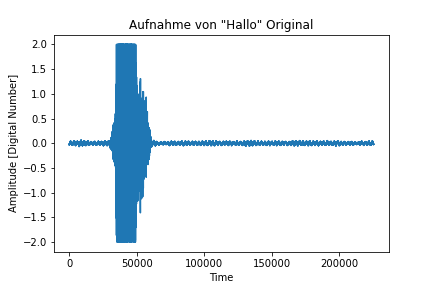
\includegraphics[width=0.75\textwidth]{media/AufnahmeHalloOriginal.png}
	\caption{Sprachaufnahme des Wortes 'Hallo'}
	\label{fig:VERSUCH_1_halloOriginal}
\end{figure}

In Abbildung \ref{fig:VERSUCH_1_halloTriggered} wird die Triggerfunktion auf das obere Signal angewendet und mit Nullen aufgefüllt.

\begin{figure}[H]
	\centering\small
	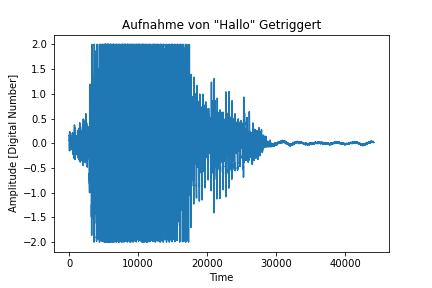
\includegraphics[width=0.75\textwidth]{media/AufnahmeHalloGetriggert.png}
	\caption{Sprachaufnahme des Wortes 'Hallo' mit Triggerfunktion}
	\label{fig:VERSUCH_1_halloTriggered}
\end{figure}

\section{Auswertung}
\label{chap:VERSUCH_1_AUSWERTUNG}
Mit der Formel
\begin{equation*}
    f = \frac{n}{M \cdot \Delta t}
\end{equation*}
kann das errechnete Spektrum im Frequenzbereich dargestellt werden. Auf der linken Seite ist das gesamte Amplitudenspektrum zu sehen und auf der rechten Seite nur einen Ausschnitt aus 2500 Samples.

\begin{figure}[H]
\centering
	\begin{subfigure}{.5\textwidth}
  		\centering
 		 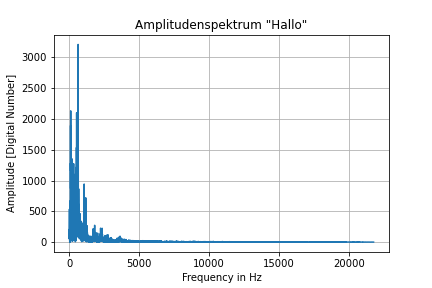
\includegraphics[width=.95\linewidth]{media/AmplitudenspektrumBreit.png}
  		\caption{Amplitudenspektrum der Sprachaufnahme}
 		 \label{fig:VERSUCH_1_sub1}
	\end{subfigure}%
	\begin{subfigure}{.5\textwidth}
  		\centering
 		 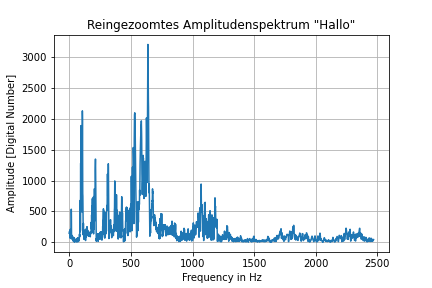
\includegraphics[width=.95\linewidth]{media/AmplitudenspektrumSchmal.png}
  		\caption{Ausschnitt des Amplitudenspektrums}
  		\label{fig:VERSUCH_1_sub2}
	\end{subfigure}
	\caption{Das Amplitudenspektrum mit der dazugehörigen Frequenz}
	\label{fig:VERSUCH_1_test}
\end{figure}

In Abbildung \ref{fig:VERSUCH_1_gauss} ist die verwendete Fensterfunktion mit einer Standardabweichung von 4 dargestellt.

\begin{figure}[H]
	\centering\small
	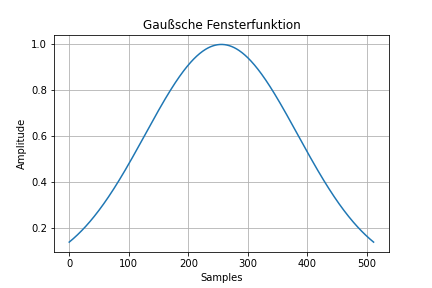
\includegraphics[width=0.75\textwidth]{media/Gauss.png}
	\caption{Gaussche Fensterfunktion mit Standardabweichung 4}
	\label{fig:VERSUCH_1_gauss}
\end{figure}

In Abbildung \ref{fig:VERSUCH_1_window} ist das durch Windowing errechnete Amplitudenspektrum zu sehen.

\begin{figure}[H]
\centering
	\begin{subfigure}{.5\textwidth}
  		\centering
 		 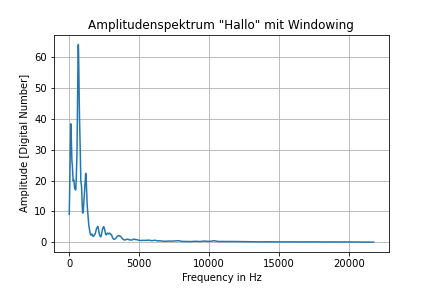
\includegraphics[width=.95\linewidth]{media/AmplitudenspektrumBreitWindow.png}
  		\caption{Amplitudenspektrum der Sprachaufnahme mit Windowing}
 		 \label{fig:VERSUCH_1_sub3}
	\end{subfigure}%
	\begin{subfigure}{.5\textwidth}
  		\centering
 		 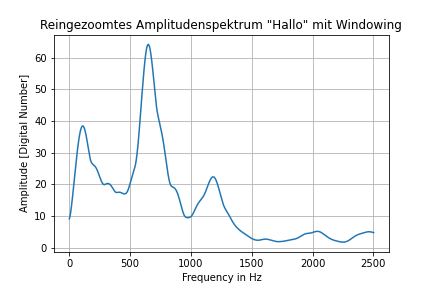
\includegraphics[width=.95\linewidth]{media/AmplitudenspektrumSchmalWindow.png}
  		\caption{Ausschnitt des Amplitudenspektrums mit Windowing}
  		\label{fig:VERSUCH_1_sub4}
	\end{subfigure}
	\caption{Das Amplitudenspektrum mit der dazugehörigen Frequenz}
	\label{fig:VERSUCH_1_window}
\end{figure}

\section{Interpretation}
\label{chap:VERSUCH_1_INTERPRETATION}

Im Vergleich von Abbildung \ref{fig:VERSUCH_1_halloOriginal} und \ref{fig:VERSUCH_1_halloTriggered} ist deutlich zu erkennen, dass der Trigger erst ab dem von uns definierten Schwellenwert ausgelöst wird und 44100 Samples lang dauert, was genau einer Sekunde entspricht.

Im Amplitundenspektrum kann man erkennen, dass es sich hierbei um kein periodisches Signal handelt. Außerdem wird dieses auf die Hälfte gekürzt, da sich das Spektrum ab der Hälfte wierderholt.

In Abbildung \ref{fig:VERSUCH_1_window} kann man schön sehen, dass das errechnete Amplitudenspektrum durch Windowing sehr ähnlich mit dem Spektrum des Originalsignals ist.

%
% CHAPTER Versuch 2
%
\chapter{Versuch 2: Spracherkennung}
\label{chap:VERSUCH_2}

\section{Fragestellung, Messprinzip, Aufbau, Messmittel}
\label{chap:VERSUCH_2_FRAGESTELLUNG}
Im zweiten Teil des Versuches sollen die Befehle 'Hoch', 'Tief', 'Links' und 'Rechts' jeweils fünf Mal aufgenommen und jeweils das Spektrum berechnet werden. Anschließend soll aus den einzelnen fünf Aufnahmen, ein Referenzsprektrum berechnet werden. Dabei ist darauf zu achten, dass alle Aufnahmen vom gleichen Sprecher gesprochen werden.

Danach werden jeweils fünf Mal die Befehle von zwei unterschiedlichen Personen aufgenommen. Im Anschluss wird von jedem Testdatensatz das Spektrum berechnet und mit den Referenzsprektren verglichen. Als Maßtab wird der Korrelationskoeffizient nach Bravais-Pearson verwendet. Umso näher der Wert bei 1 ist, desto größer ist die Ähnlichkeit zu dem Referenzspektrum.

Zum Schluss soll noch die Detektions- und Fehlerrate angegeben werden.
\newpage
\section{Messwerte}
\label{chap:VERSUCH_2_MESSWERTE}
In Abbildung \ref{fig:VERSUCH_2_firstSpectrums} werden die Spektren der ersten Aufnahmen der jeweiligen Befehle dargestellt. Die Spektren wurden ebenfalls durch das Windowing berechnet.

\begin{figure}[H]
\centering
	\begin{subfigure}{.5\textwidth}
  		\centering
 		 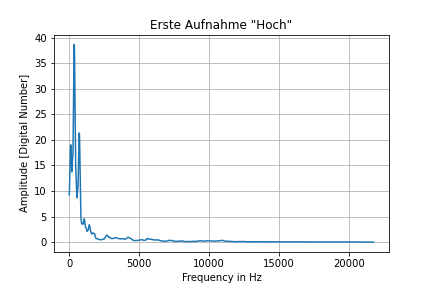
\includegraphics[width=.95\linewidth]{media/ersteAufnahmeHoch.png}
  		\caption{Spektrum vom Befehl "Hoch"}
 		 \label{fig:VERSUCH_2_sub1}
	\end{subfigure}%
	\begin{subfigure}{.5\textwidth}
  		\centering
 		 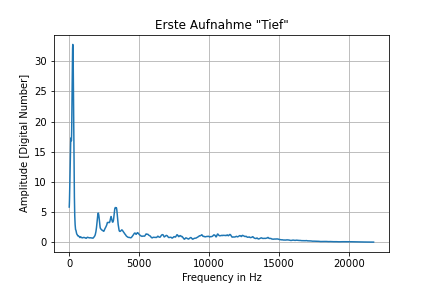
\includegraphics[width=.95\linewidth]{media/ersteAufnahmeTief.png}
  		\caption{Spektrum vom Befehl "Tief"}
  		\label{fig:VERSUCH_2_sub2}
	\end{subfigure}
	\begin{subfigure}{.5\textwidth}
  		\centering
 		 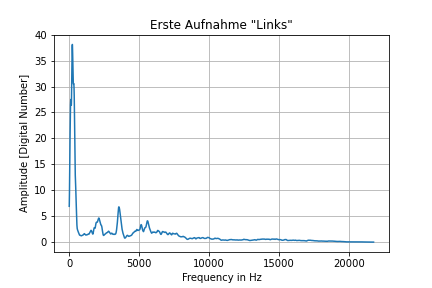
\includegraphics[width=.95\linewidth]{media/ersteAufnahmeLinks.png}
  		\caption{Spektrum vom Befehl "Links"}
  		\label{fig:VERSUCH_2_sub3}
	\end{subfigure}%
	\begin{subfigure}{.5\textwidth}
  		\centering
 		 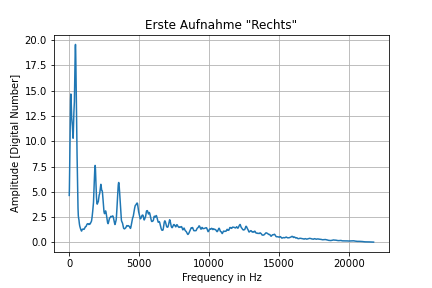
\includegraphics[width=.95\linewidth]{media/ersteAufnahmeRechts.png}
  		\caption{Spektrum vom Befehl "Rechts"}
  		\label{fig:VERSUCH_2_sub4}
	\end{subfigure}
	\caption{Die Spektren der ersten Aufnahmen}
	\label{fig:VERSUCH_2_firstSpectrums}
\end{figure}
\newpage
\section{Auswertung}
\label{chap:VERSUCH_2_AUSWERTUNG}
In Abbildung \ref{fig:VERSUCH_2_referencsSpecs} werden die Referenzsprektren der vier Befehle dargestellt. Das Referenzspektrum haben wir wie folgt berechnet: Zuerst haben wir von jedem der fünf Aufnahmen pro Befehl, das Spektrum mithilfe von Windowing berechnet und anschließend aus den fünf Spektren den Mittelwert daraus genommen.

\begin{figure}[H]
\centering
	\begin{subfigure}{.5\textwidth}
  		\centering
 		 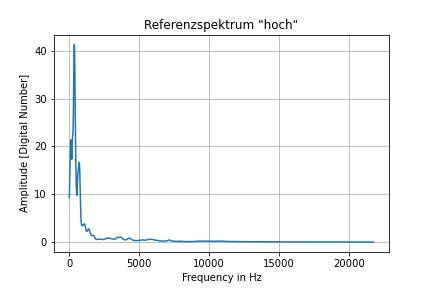
\includegraphics[width=.95\linewidth]{media/ReferenzspektrumHoch.png}
  		\caption{Referenzspektrum vom Befehl "Hoch"}
 		 \label{fig:VERSUCH_2_sub5}
	\end{subfigure}%
	\begin{subfigure}{.5\textwidth}
  		\centering
 		 \includegraphics[width=.95\linewidth]{media/ReferenzspektrumTief.png}
  		\caption{Referenzspektrum vom Befehl "Tief"}
  		\label{fig:VERSUCH_2_sub6}
	\end{subfigure}
	\begin{subfigure}{.5\textwidth}
  		\centering
 		 \includegraphics[width=.95\linewidth]{media/ReferenzspektrumLinks.png}
  		\caption{Referenzspektrum vom Befehl "Links"}
  		\label{fig:VERSUCH_2_sub7}
	\end{subfigure}%
	\begin{subfigure}{.5\textwidth}
  		\centering
 		 \includegraphics[width=.95\linewidth]{media/ReferenzspektrumRechts.png}
  		\caption{Referenzspektrum vom Befehl "Rechts"}
  		\label{fig:VERSUCH_2_sub8}
	\end{subfigure}
	\caption{Die Referenzsprektren der Befehle}
	\label{fig:VERSUCH_2_referencsSpecs}
\end{figure}

In den nachffolgenden Tabellen sind die Testdatensätze zu sehen, die mit dem Referenzspektren verglichen wurden. In der linken Spalte ist der Name des Testdatensatzes beschrieben. In der zweiten Spalte steht der Korrelationskoeffiezient zu dem erkannten Befehl. Der erkannte Befehl befindet sich in der dritten Spalte. Ganz rechts in der Tabelle steht, ob die Schätzung des Python Programms korrekt war.

\newpage
In Tabelle \ref{fig:VERSUCH_2_person1} sind die Ergebnisse von Person 1 (Sprecher der Referenzspektren) ersichtlich.

\begin{table}[H]
\centering
\begin{tabular}{|l|l|l||l|}
\hline
\multicolumn{1}{|c|}{\textbf{Befehl}} & \textbf{Korrelationskoeffizient} & \textbf{Geschätzt} & \textbf{Erkannt?} \\ \hline
hoch1\textunderscore training.csv			& 0.6392205098106617			& Hoch			& Ja		\\ \hline
hoch2\textunderscore training.csv			& 0.6908852507975607			& Hoch			& Ja		\\ \hline
hoch3\textunderscore training.csv			& 0.7369898355976126			& Hoch			& Ja		\\ \hline
hoch4\textunderscore training.csv			& 0.6531021613772101			& Hoch			& Ja		\\ \hline
hoch5\textunderscore training.csv			& 0.5846061001105898			& Hoch			& Ja		\\ \hline
tief1\textunderscore training.csv			& 0.6917387323004587			& Tief			& Ja		\\ \hline
tief2\textunderscore training.csv			& 0.597228535138889			& Tief			& Ja		\\ \hline
tief3\textunderscore training.csv			& 0.5857716921817915			& Tief			& Ja		\\ \hline
tief4\textunderscore training.csv			& 0.5184803106129552			& Tief			& Ja		\\ \hline
tief5\textunderscore training.csv			& 0.4920849692590793			& Tief			& Ja		\\ \hline
links1\textunderscore training.csv			& 0.683875009035533			& Links			& Ja		\\ \hline
links2\textunderscore training.csv			& 0.6877934469896636			& Links			& Ja		\\ \hline
links3\textunderscore training.csv			& 0.6764595830513251			& Links			& Ja		\\ \hline
links4\textunderscore training.csv			& 0.7451023996899163			& Links			& Ja		\\ \hline
links5\textunderscore training.csv			& 0.6901293090260275			& Links			& Ja		\\ \hline
rechts1\textunderscore training.csv			& 0.7439299919720688			& Rechts			& Ja		\\ \hline
rechts2\textunderscore training.csv			& 0.6660542874986765			& Rechts			& Ja		\\ \hline
rechts3\textunderscore training.csv			& 0.5576880105772456			& Rechts			& Ja		\\ \hline
rechts4\textunderscore training.csv			& 0.6184389154587102			& Rechts			& Ja		\\ \hline
rechts5\textunderscore training.csv			& 0.6147002078697453			& Rechts			& Ja		\\ \hline
\end{tabular}
\caption{Korrelationskoeffizienten von Person 1 bzw. des Spechers der Referenzspektren}
\label{fig:VERSUCH_2_person1}
\end{table}

\newpage
In Tabelle \ref{fig:VERSUCH_2_person2} sind die Ergebnisse von Person 2 zu sehen.

\begin{table}[H]
\centering
\begin{tabular}{|l|l|l||l|}
\hline
\multicolumn{1}{|c|}{\textbf{Befehl}} & \textbf{Korrelationskoeffizient} & \textbf{Geschätzt} & \textbf{Erkannt?} \\ \hline
hoch1\textunderscore training.csv			& 0.5617656486091793			& Hoch			& Ja		\\ \hline
hoch2\textunderscore training.csv			& 0.6034073877089225			& Hoch			& Ja		\\ \hline
hoch3\textunderscore training.csv			& 0.6609418303129206			& Hoch			& Ja		\\ \hline
hoch4\textunderscore training.csv			& 0.5627980823380955			& Hoch			& Ja		\\ \hline
hoch5\textunderscore training.csv			& 0.60474571557112			& Hoch			& Ja		\\ \hline
tief1\textunderscore training.csv			& 0.796451643049229			& Links			& Nein		\\ \hline
tief2\textunderscore training.csv			& 0.7883298868956207			& Links			& Nein		\\ \hline
tief3\textunderscore training.csv			& 0.7931331080053363			& Links			& Nein		\\ \hline
tief4\textunderscore training.csv			& 0.784277955016512			& Links			& Nein		\\ \hline
tief5\textunderscore training.csv			& 0.7574809465314387			& Links			& Nein		\\ \hline
links1\textunderscore training.csv			& 0.5950941597762736			& Rechts			& Nein		\\ \hline
links2\textunderscore training.csv			& 0.5975798374627092			& Rechts			& Nein		\\ \hline
links3\textunderscore training.csv			& 0.6181404787738591			& Rechts			& Nein		\\ \hline
links4\textunderscore training.csv			& 0.653205184868384			& Rechts			& Nein		\\ \hline
links5\textunderscore training.csv			& 0.637358727357185			& Rechts			& Nein		\\ \hline
rechts1\textunderscore training.csv			& 0.5274964804138591			& Rechts			& Ja		\\ \hline
rechts2\textunderscore training.csv			& 0.5182675549402136			& Rechts			& Ja		\\ \hline
rechts3\textunderscore training.csv			& 0.4888507104169534			& Rechts			& Ja		\\ \hline
rechts4\textunderscore training.csv			& 0.46684747064840704			& Rechts			& Ja		\\ \hline
rechts5\textunderscore training.csv			& 0.47841493852970246			& Rechts			& Ja		\\ \hline
\end{tabular}
\caption{Korrelationskoeffizienten von Person 2}
\label{fig:VERSUCH_2_person2}
\end{table}

\begin{table}[H]
\centering
\begin{tabular}{|l|l|l|}
\hline
\multicolumn{1}{|c|}{\textbf{Person}} & \textbf{Detektionsrate} & \textbf{Fehlerrate} \\ \hline
Person 1     & 100\%         & 0\%       \\ \hline
Person 2     & 50\%         & 50\%       \\ \hline
\end{tabular}
\caption{Detektions- und Fehlerrate der Personen}
\label{fig:VERSUCH_2_rates}
\end{table}
\newpage
\section{Interpretation}
\label{chap:VERSUCH_2_INTERPRETATION}

Die Ergebnisse von Person 1, welcher der Sprecher der Referenzspektren war, sind wie zu erwarten, mit einer Detektionsrate von 100\% einwandfrei. Jedoch sieht das bei Person 2 anders aus, da hier die Detektionsrate nur bei 50\% liegt. Beispielweise wurde anstatt 'Tief' der Befehl 'Links' erkannt, was sich darauf zurückzuführen lässt, dass die Referenzspektren von 'Tief' und 'Links' in den niedriegen Frequenzen sehr identisch sind und dadurch stark korrelieren.

Schlussfolgernd lässt sich die Erkenntiss schließen, dass wenn man sich ein Spracherkenner für den privaten Gebrauch bauen möchte, dies eine gute Methode ist und sehenswerte Ergebnisse liefert. Jedoch ist diese Methode nicht für die breite Masse geeignet, da in unserem Beispiel eine Detektionsrate von 50\% zu ungenau ist, wenn andere Stimmen mit ins Spiel kommen. Eventuell hätte der Spracherkenner bessere Ergebnisse geliefert, wenn wir für die Berechnung der Referenzspektren noch mehr Testdatensätze verwendet hätten, wie auch verschiedene Sprecher.

%
% CHAPTER Anhang
%
\renewcommand\thesection{A.\arabic{section}}
\renewcommand\thesubsection{\thesection.\arabic{subsection}}

\chapter*{Anhang}
\label{chap:APPENDIX}
\addcontentsline{toc}{chapter}{Anhang}
%\setcounter{chapter}{0}
\addtocounter{chapter}{1}
\setcounter{section}{0}

\section{Quellcode}
\label{chap:APPENDIX_SOURCECODE}

\subsection{Quellcode Versuch 1}
\label{chap:APPENDIX_SOURCECODE_V1}
\lstinputlisting[style=PYTHON, frame=single, caption=Skript Versuch 1a, captionpos=b, label=lst:APPENDIX_SOURCECODE_PLOT]{code/1.1.py}
\lstinputlisting[style=PYTHON, frame=single, caption=Skript Versuch 1b, captionpos=b, label=lst:APPENDIX_SOURCECODE_PLOT]{code/1.2.py}
\lstinputlisting[style=PYTHON, frame=single, caption=Skript Versuch 1c, captionpos=b, label=lst:APPENDIX_SOURCECODE_PLOT]{code/1.3.py}
\lstinputlisting[style=PYTHON, frame=single, caption=Skript Versuch 1d, captionpos=b, label=lst:APPENDIX_SOURCECODE_PLOT]{code/1.4.py}
\newpage
\subsection{Quellcode Versuch 2}
\label{chap:APPENDIX_SOURCECODE_V2}
\lstinputlisting[style=PYTHON, frame=single, caption=Skript Versuch 2a, captionpos=b, label=lst:APPENDIX_SOURCECODE_PLOT]{code/2.1.py}
\lstinputlisting[style=PYTHON, frame=single, caption=Skript Versuch 2c+d, captionpos=b, label=lst:APPENDIX_SOURCECODE_PLOT]{code/2.3.py}

\end{document}
%------------------------------------
% ╔═╗╔╗╔╔╦╗  ╔╦╗╔═╗╔═╗╦ ╦╔╦╗╔═╗╔╗╔╔╦╗
% ║╣ ║║║ ║║   ║║║ ║║  ║ ║║║║║╣ ║║║ ║
% ╚═╝╝╚╝═╩╝  ═╩╝╚═╝╚═╝╚═╝╩ ╩╚═╝╝╚╝ ╩
%------------------------------------